El PBS, \textit{Product Breakdown Structure}, es una estructura jerárquica que descompone el proyecto en los productos que se deben entregar para cumplir 
con los objetivos del proyecto. 
En las siguientes secciones se detallan los productos que se deben entregar en el proyecto BidMon Universe.

\subsubsection{PBS. Visión general}
En la \coloredUnderline{\hyperlink{fig:5_PBS-Vision-General}{Figura \ref*{fig:5_PBS-Vision-General}: \nameref*{fig:5_PBS-Vision-General}}} se muestran los productos de alto nivel que se deben entregar en el proyecto BidMon Universe. 
En las siguientes secciones, se entrará en detalle en cada uno de los productos.

\begin{figure}[H]
    \hypertarget{fig:5_PBS-Vision-General}{}
    \centering
    \includegraphics[width=0.5\linewidth]{figures/5-PBS/5_PBS-Vision-General.png}
    \caption{PBS. Visión general}
    \label{fig:5_PBS-Vision-General}
\end{figure}


\subsubsection{PBS. Análisis del sistema}
En la \coloredUnderline{\hyperlink{fig:5_PBS-Analisis-Sistema}{Figura \ref*{fig:5_PBS-Analisis-Sistema}: \nameref*{fig:5_PBS-Analisis-Sistema}}}, se detallan los productos que se deben entregar en la fase de análisis del sistema.
\begin{figure}[H]
    \hypertarget{fig:5_PBS-Analisis-Sistema}{}
    \centering
    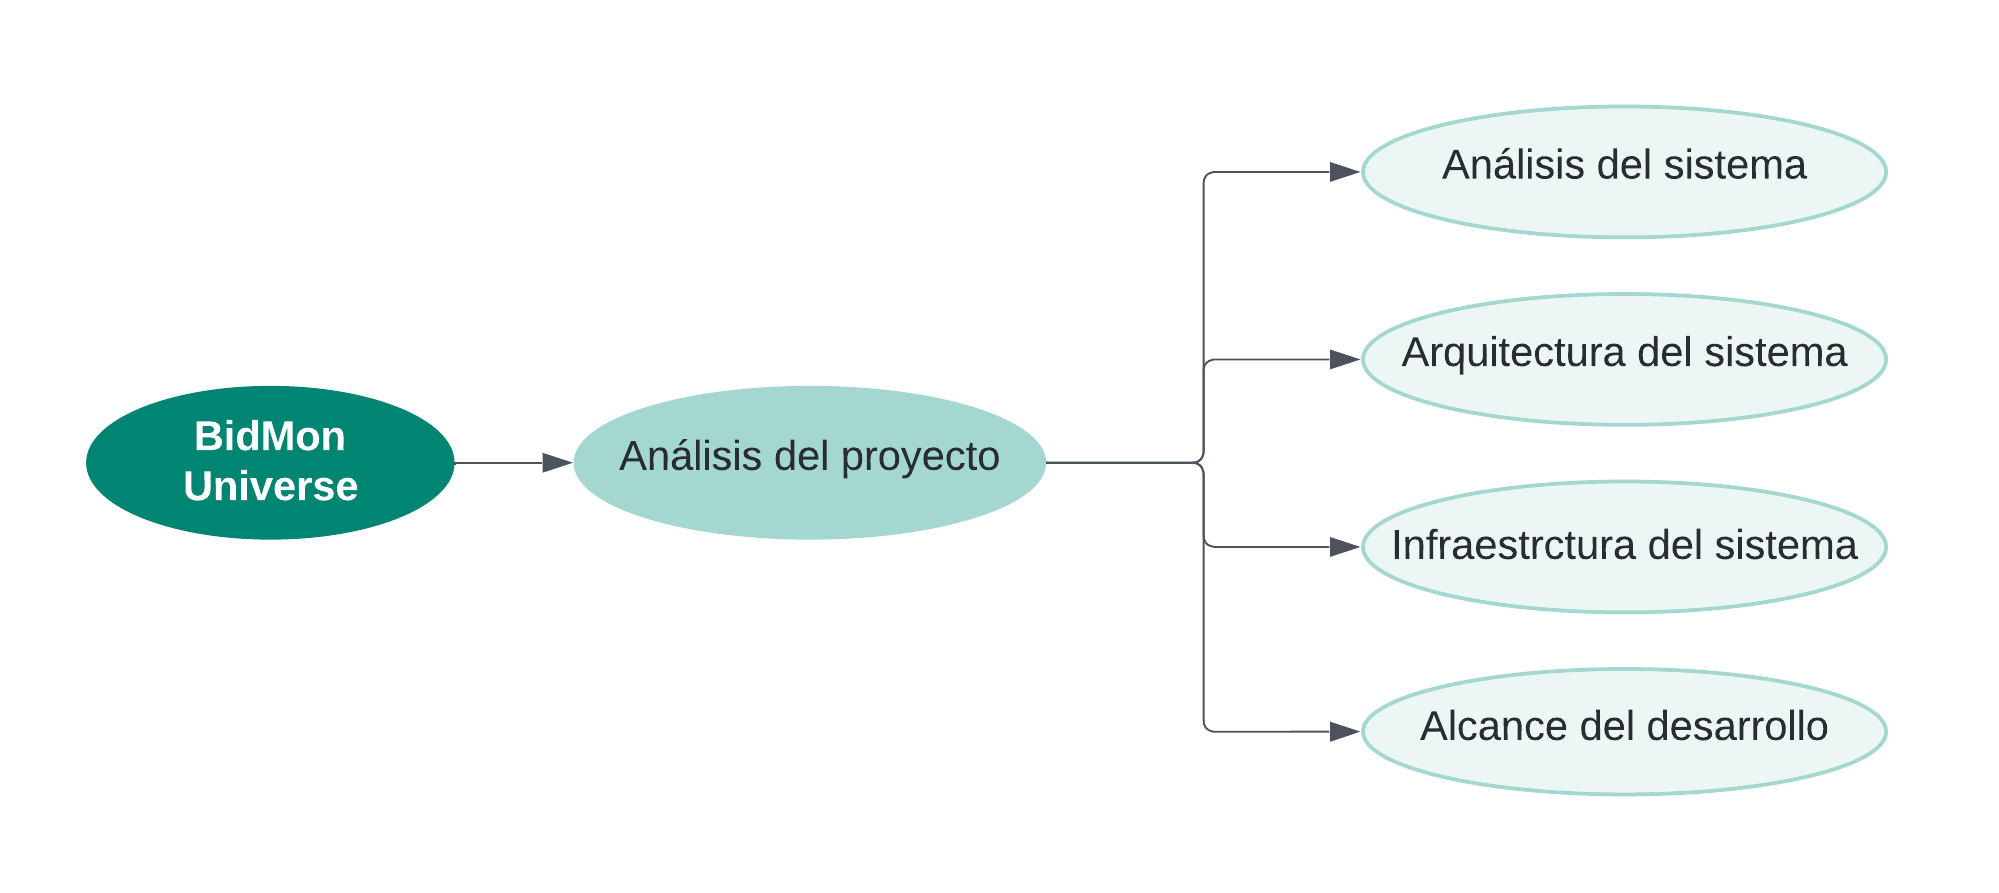
\includegraphics[width=0.7\linewidth]{figures/5-PBS/5_PBS-Analisis.png}
    \caption{PBS. Análisis del sistema}
    \label{fig:5_PBS-Analisis-Sistema}
\end{figure}

\subsubsection{PBS. Seguimiento del sistema}
En esta fase se detallan los productos que se obtienen en la fase de segumiento del proyecto, principalmente documentación e informes como se muestra en la \coloredUnderline{\hyperlink{fig:5_PBS-Seguimiento-Sistema}{Figura \ref*{fig:5_PBS-Seguimiento-Sistema}: \nameref*{fig:5_PBS-Seguimiento-Sistema}}}.
\begin{figure}[H]
    \hypertarget{fig:5_PBS-Seguimiento-Sistema}{}
    \centering
    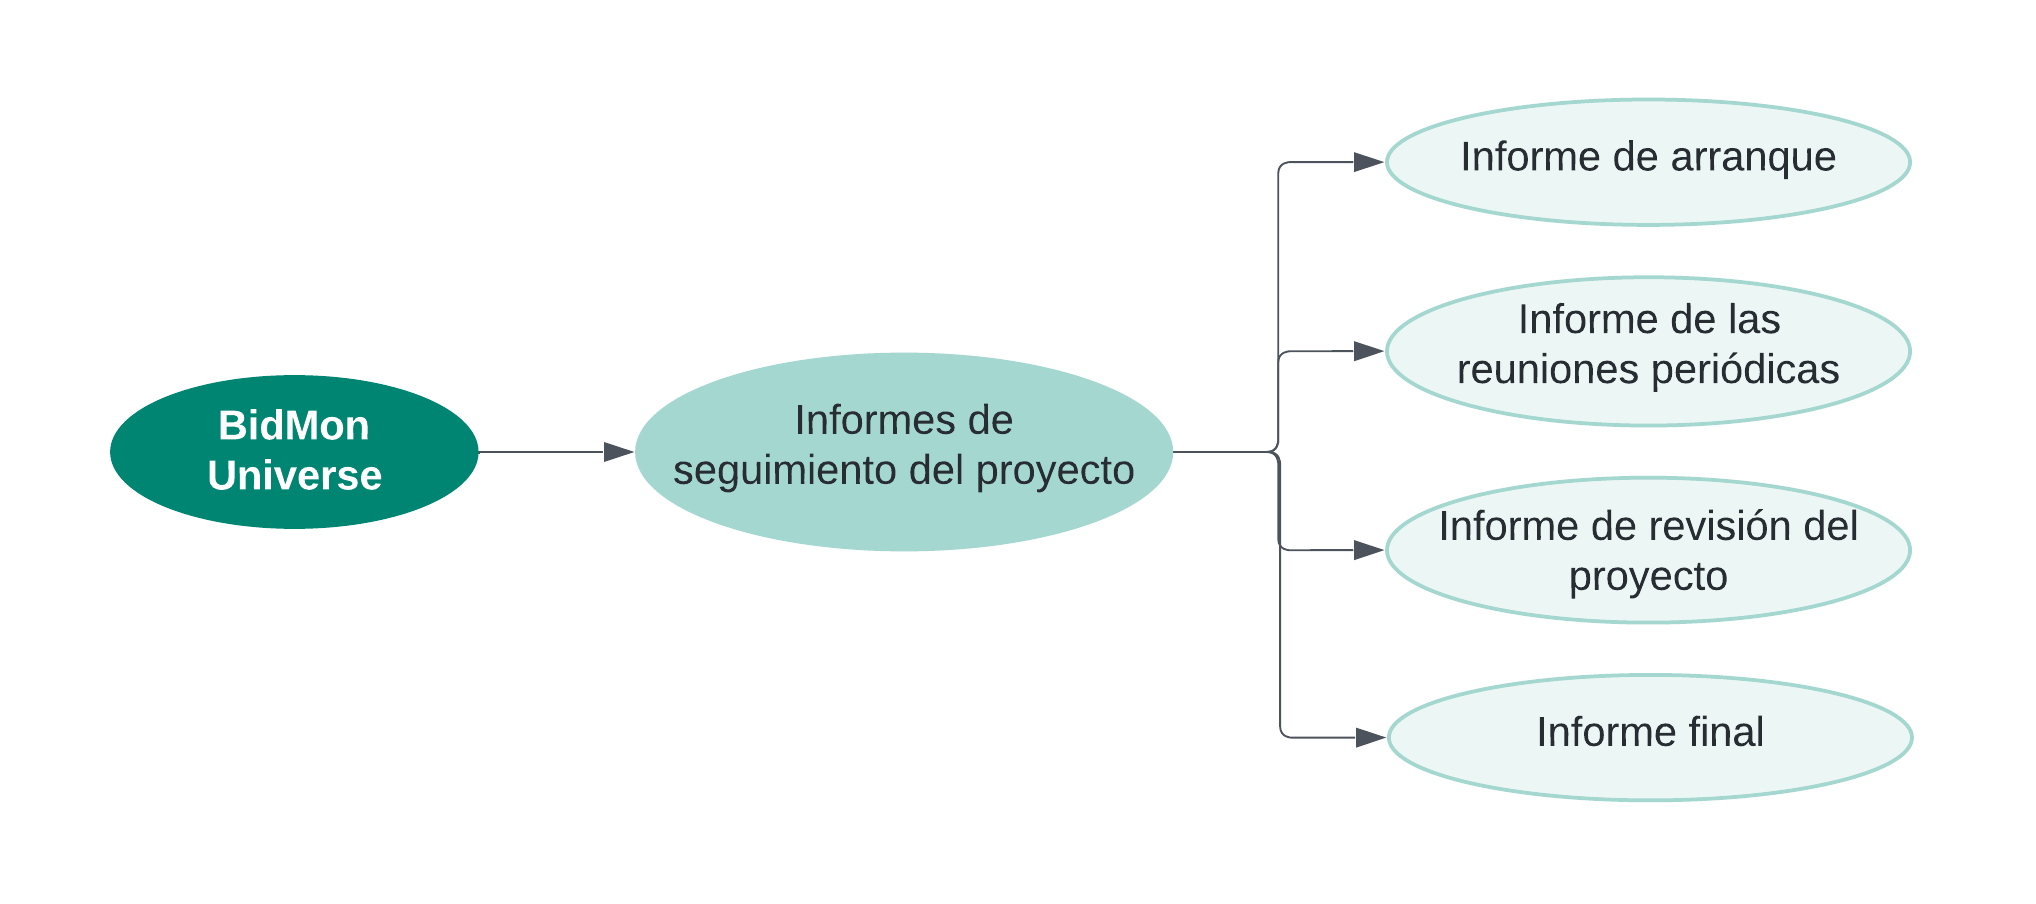
\includegraphics[width=0.7\linewidth]{figures/5-PBS/5_PBS-Seguimiento.png}
    \caption{PBS. Seguimiento del sistema}
    \label{fig:5_PBS-Seguimiento-Sistema}
\end{figure}

\subsubsection{PBS. Diseño del sistema}
En la \coloredUnderline{\hyperlink{fig:5_PBS-Diseño-Sistema}{Figura \ref*{fig:5_PBS-Diseño-Sistema}: \nameref*{fig:5_PBS-Diseño-Sistema}}}, se detallan los productos que se deben entregar en la fase de diseño del sistema.
\begin{figure}[H]
    \hypertarget{fig:5_PBS-Diseño-Sistema}{}
    \centering
    \includegraphics[width=0.9\linewidth]{figures/5-PBS/5_PBS-Diseno.png}
    \caption{PBS. Diseño del sistema}
    \label{fig:5_PBS-Diseño-Sistema}
\end{figure}

\subsubsection{PBS. Implementación del sistema}
En la \coloredUnderline{\hyperlink{fig:5_PBS-Implementación-Sistema}{Figura \ref*{fig:5_PBS-Implementación-Sistema}: \nameref*{fig:5_PBS-Implementación-Sistema}}}, se detallan los productos a realizar en la fase de implementación del sistema.
\begin{figure}[H]
    \hypertarget{fig:5_PBS-Implementación-Sistema}{}
    \centering
    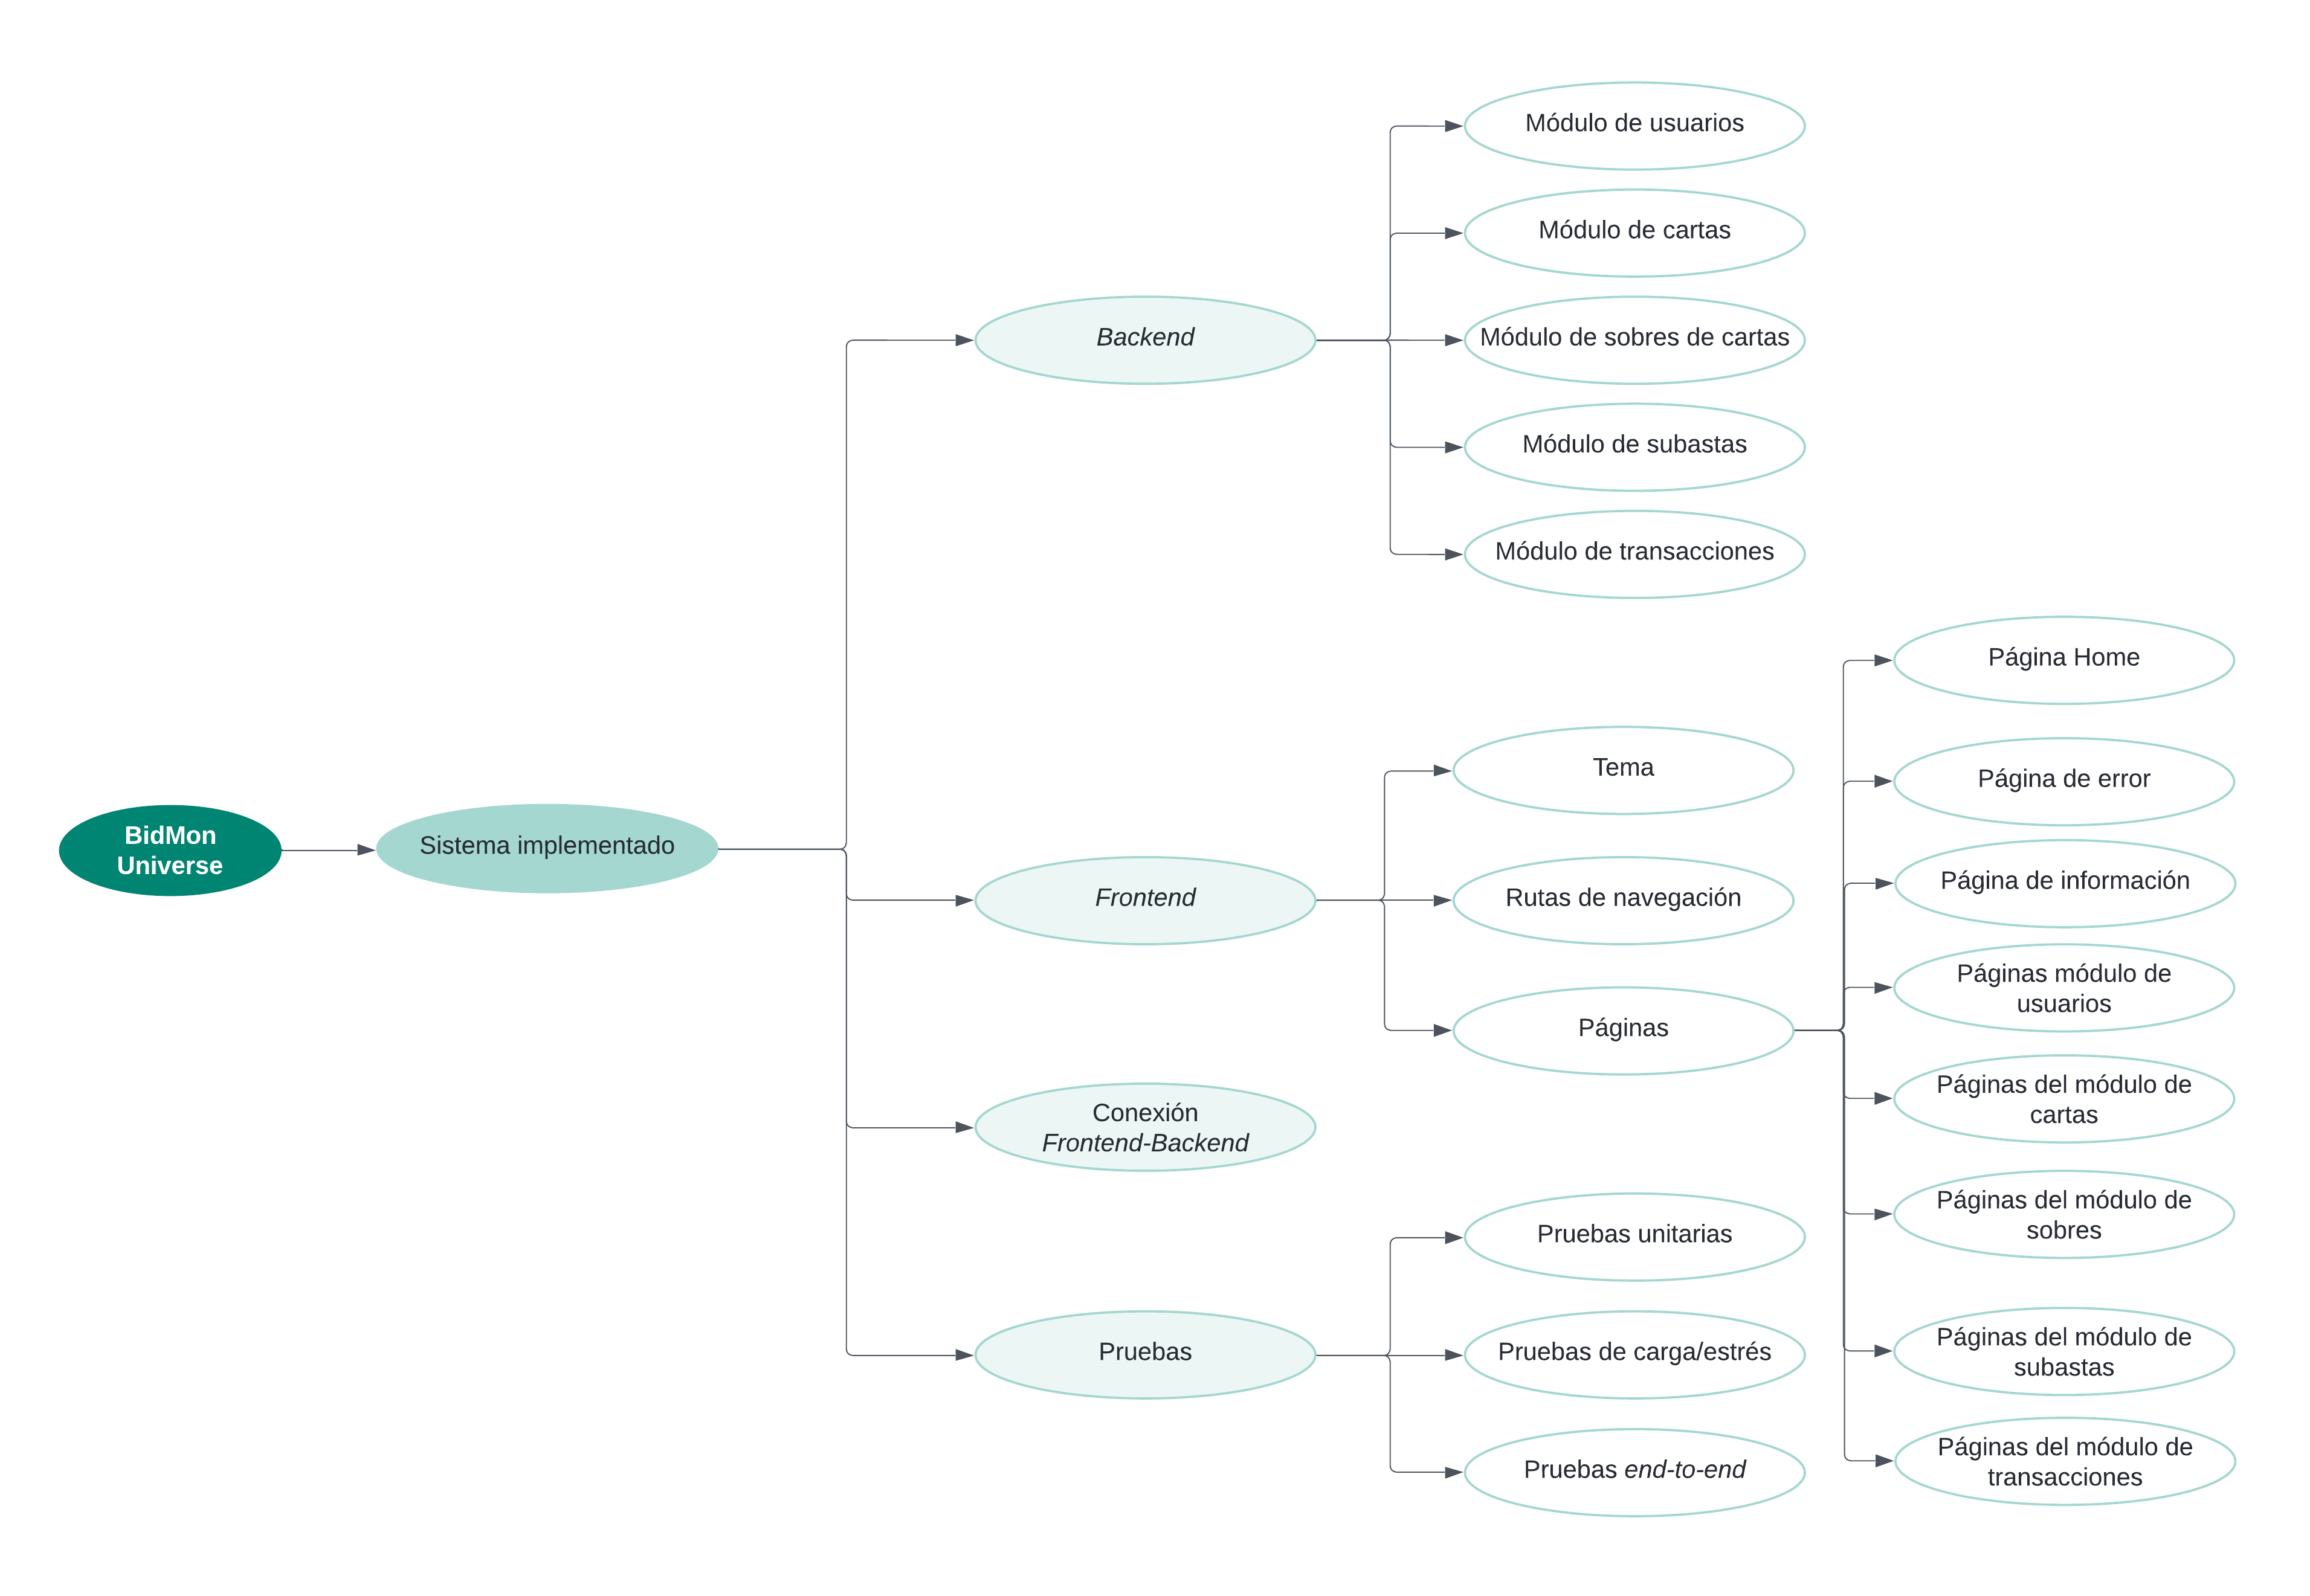
\includegraphics[width=0.9\linewidth]{figures/5-PBS/5_PBS-Implementacion.png}
    \caption{PBS. Implementación del sistema}
    \label{fig:5_PBS-Implementación-Sistema}
\end{figure}

\subsubsection{PBS. Pruebas del sistema}
En la fase de pruebas del sistema se obtienen como productos los resultados de la ejecución de dichas pruebas.
\begin{figure}[H]
    \hypertarget{fig:5_PBS-Pruebas}{}
    \centering
    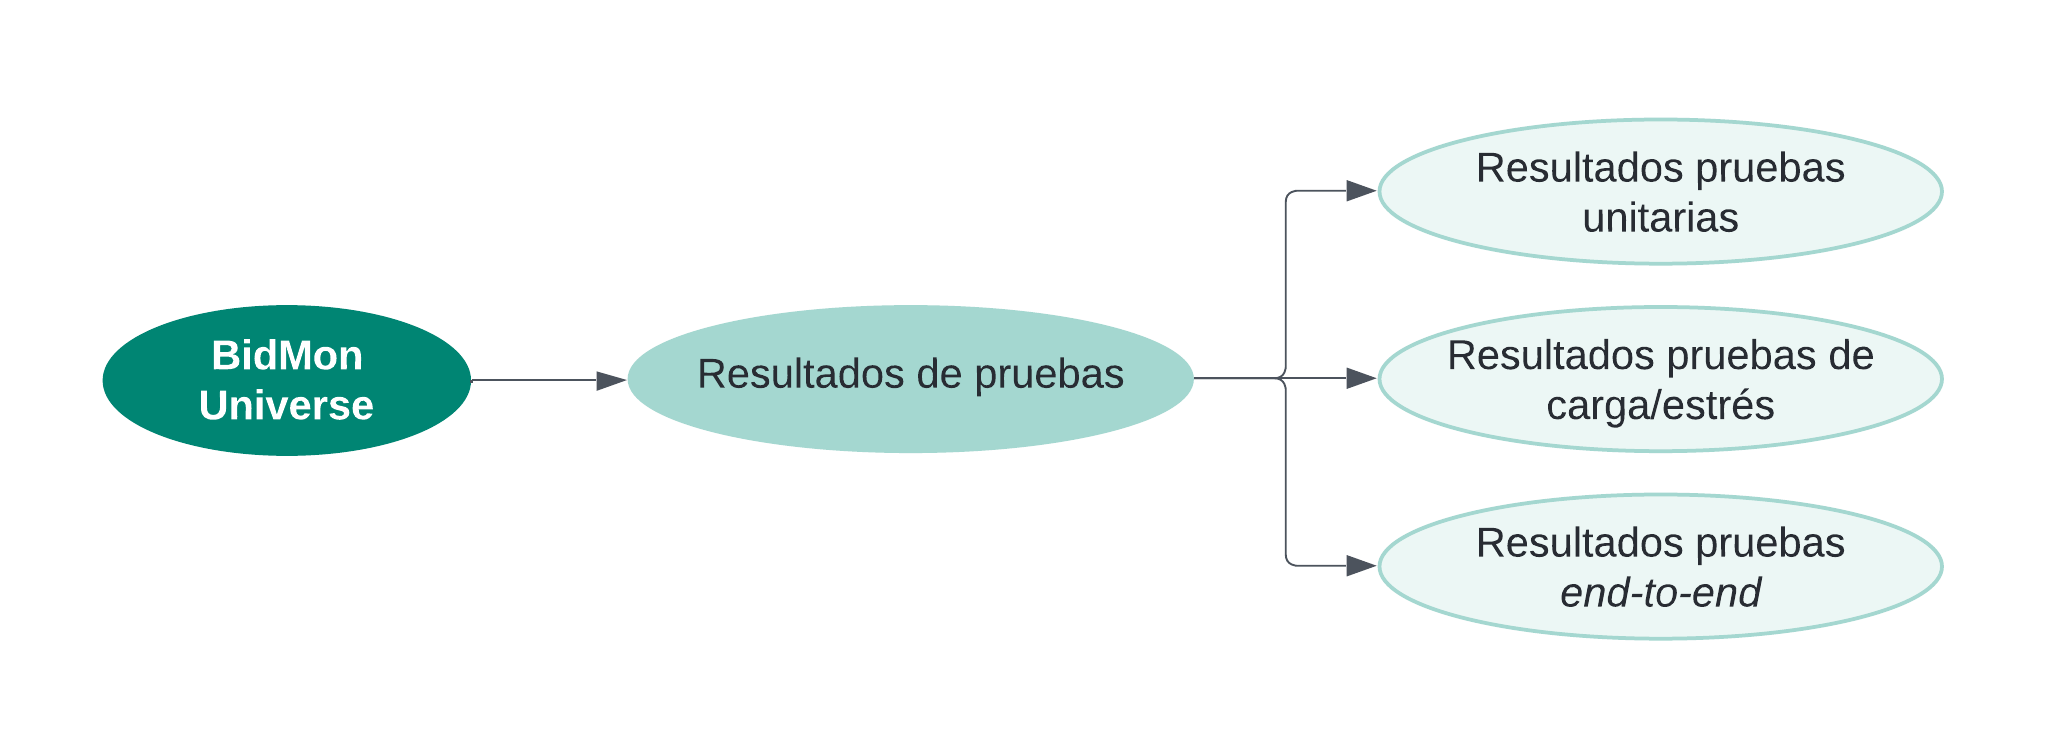
\includegraphics[width=0.7\linewidth]{figures/5-PBS/5_PBS-Pruebas.png}
    \caption{PBS. Pruebas del sistema}
    \label{fig:5_PBS-Pruebas}
\end{figure}

\subsubsection{PBS. Despliegue del sistema}
En la fase de despliegue del sistema se obtiene como producto el sistema desplegado y en funcionamiento.
\begin{figure}[H]
    \hypertarget{fig:5_PBS-Despliegue-Sistema}{}
    \centering
    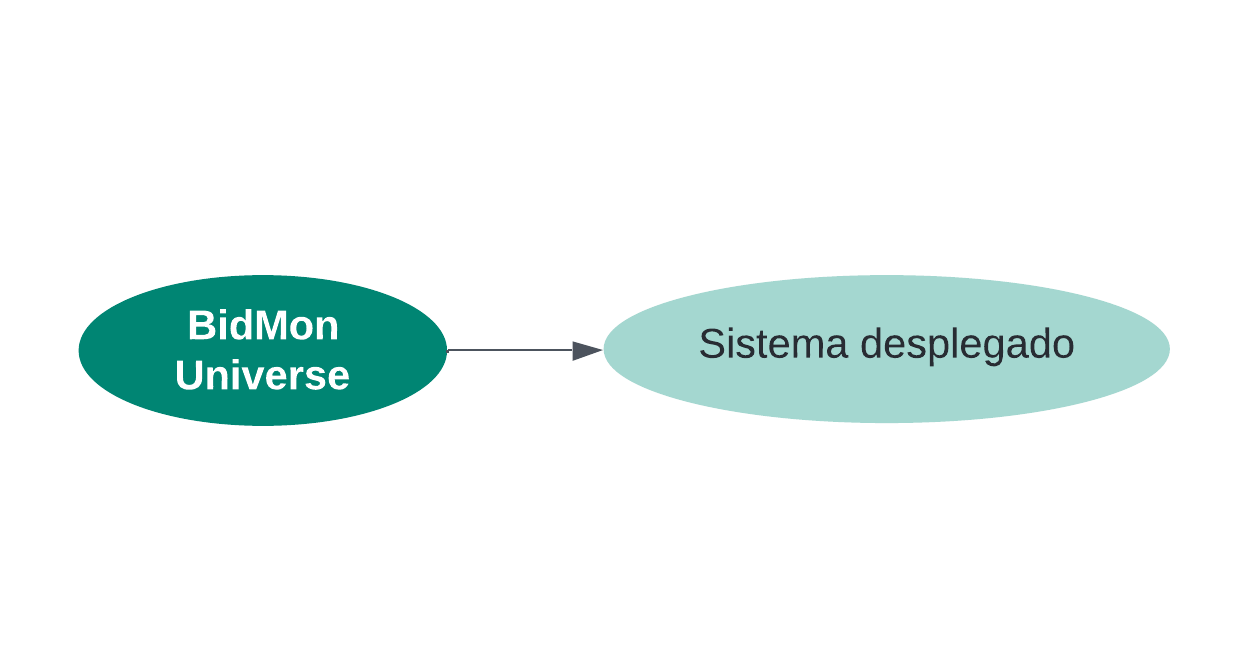
\includegraphics[width=0.7\linewidth]{figures/5-PBS/5_PBS-Despliegue.png}
    \caption{PBS. Despliegue del sistema}
    \label{fig:5_PBS-Despliegue-Sistema}
\end{figure}


\subsubsection{PBS. Documentación del sistema}
En la fase de documentación del sistema se obtienen como productos los documentos técnicos que describen el proyecto junto con los anexos.
\begin{figure}[H]
    \hypertarget{fig:5_PBS-Documentación-Sistema}{}
    \centering
    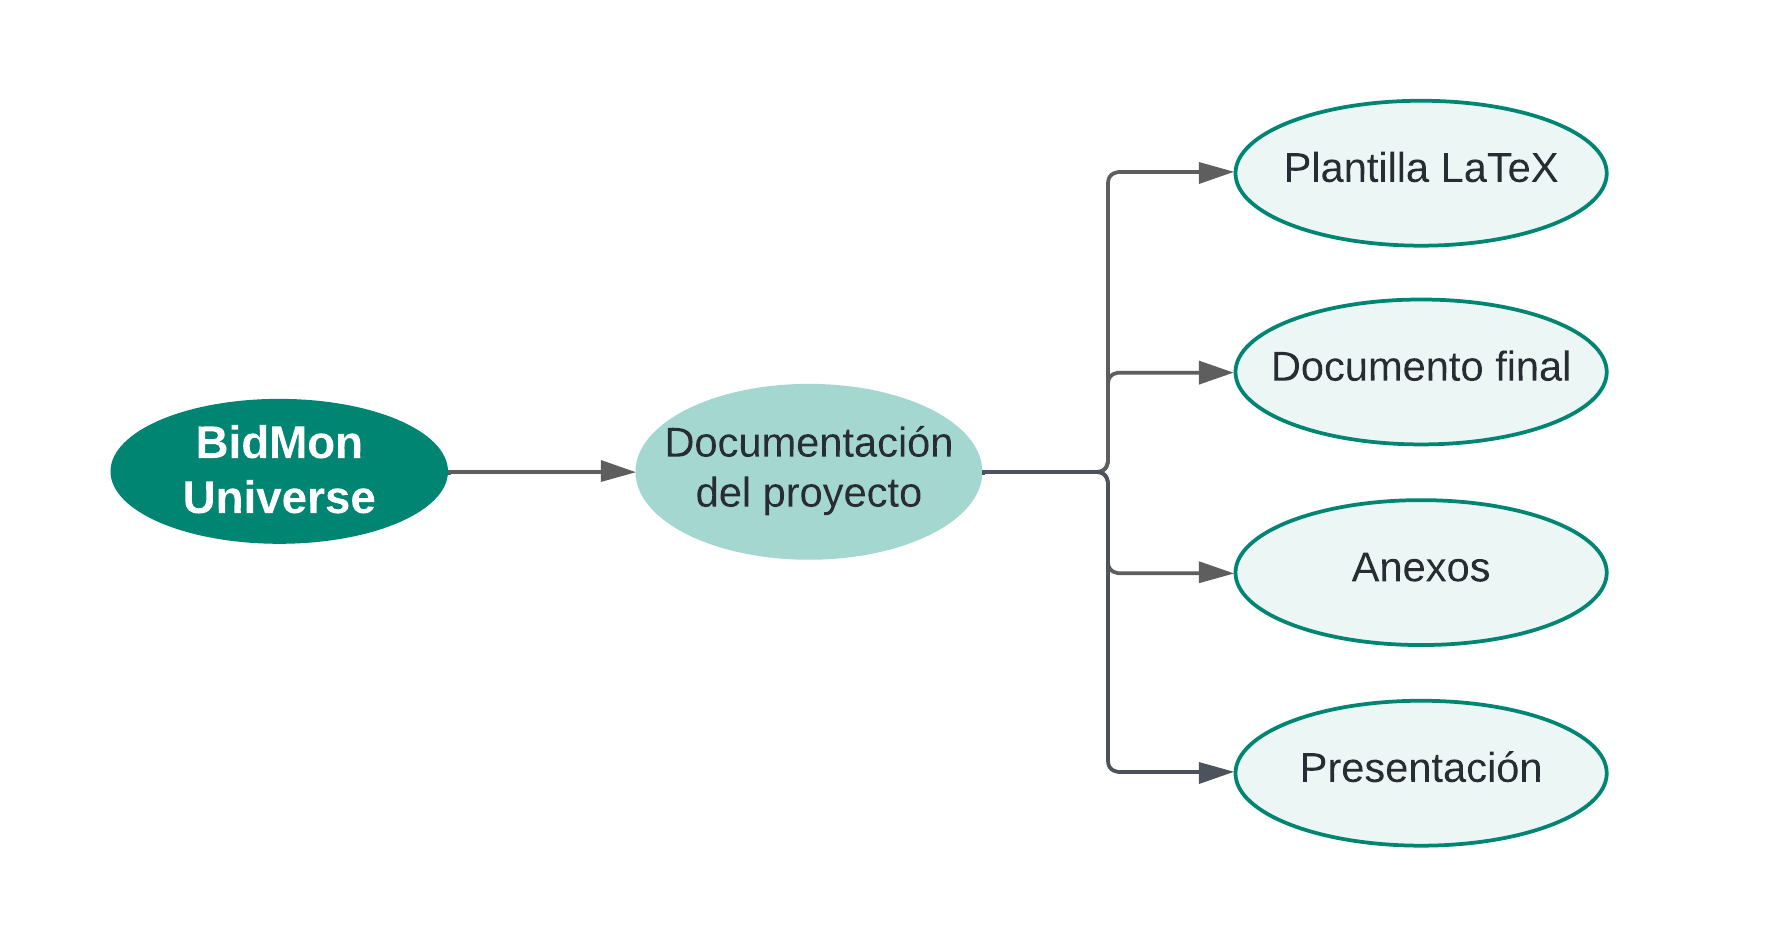
\includegraphics[width=0.7\linewidth]{figures/5-PBS/5_PBS-Documentacion.png}
    \caption{PBS. Documentación del sistema}
    \label{fig:5_PBS-Documentación-Sistema}
\end{figure}

